
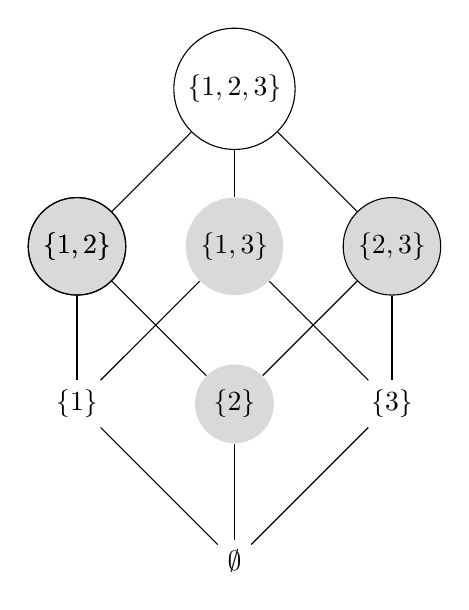
\begin{tikzpicture}%[scale=1.5, transform shape, every node/.style={draw, circle, minimum size=1cm}]
    % Define the subsets
    \node (empty) at (0,0) {$\emptyset$};
    \node (1) at (-2,2) {$\{1\}$};
    \node[circle, minimum size=1cm, fill=gray!30] (2) at (0,2) {$\{2\}$};
    \node (3) at (2,2) {$\{3\}$};
    \node[draw, circle, minimum size=1cm, fill=gray!30] (12) at (-2,4) {$\{1, 2\}$};
    \node[circle, minimum size=1cm, fill=gray!30] (13) at (0,4) {$\{1, 3\}$};
    \node[draw, circle, minimum size=1cm, fill=gray!30] (23) at (2,4) {$\{2, 3\}$};
    \node[draw, circle, minimum size=1cm] (123) at (0,6) {$\{1, 2, 3\}$};
    
    \node[draw, circle, minimum size=1cm] (12) at (-2,4) {$\{1, 2\}$};

    % Draw the edges
    \draw (empty) -- (1);
    \draw (empty) -- (2);
    \draw (empty) -- (3);
    \draw (1) -- (12);
    \draw (1) -- (13);
    \draw (2) -- (12);
    \draw (2) -- (23);
    \draw (3) -- (13);
    \draw (3) -- (23);
    \draw (12) -- (123);
    \draw (13) -- (123);
    \draw (23) -- (123);
\end{tikzpicture}

